\input{mmd-article-header}
\def\mytitle{Project Report}
\def\myauthor{Adam Whiteside \& Scott Richie \& Andrew Vadnal \& Terence Siganakis}
\def\mydate{2012-05-31}
\def\latexmode{memoir}
\input{mmd-article-begin-doc}
\part{Introduction}
\label{introduction}

\chapter{Introduction}
\label{introduction}

This report outlines the architecure, design and implementation details of The Grid, a distributed grid computing software package. The Grid allows for the distribution and exectution of self-contained executable files across a heterogenous grid, allowing users of the software to optimise the running of their jobs based on their deadline and any cost restraints. This software package includes a number of different scheduling algorithms that can be used depending on the type of jobs The Grid will be used for.

\part{Architecture}
\label{architecture}

\chapter{Architecture}
\label{architecture}

The architecture of The Grid involves 3 key components: The Master, The Client and The Node.

\section{The Client}
\label{theclient}

The Client is what the user interacts with to execute jobs on The Grid. The Client sends an executables and input files to The Master, and then also requests and downloads the output files from The Master when the job has completed. The Client can be installed in any location as it connects to The Master remotely. The Client can be reimplemented in any language as long as it follows the expected API to comunicate with The Master and authenticates with a trusted username and password.

\section{The Node}
\label{thenode}

The Node is the workhorse of The Grid. Many computation nodes are setup with The Node, each of which connects to The Master. After specifying the number of cores available for use, and the cost to use the node, each instance is then ready to accept jobs delegated to it by The Master. The Node is responsible for the execution of delegated jobs, then informing The Master as jobs are finished, and sending the output and error files of the job back to The Master.

\section{The Master}
\label{themaster}

The Master is the central component of The Grid. All communication between The Client and The Nodes goes through The Master. The Master accepts job requests from The Client and then adds them to an internal queue. It then determines which jobs should be run and on which node in The Grid. It keeps track of which jobs are on which nodes and what the status of each job is. 

\part{Design}
\label{design}

\chapter{Design}
\label{design}

\begin{figure}[htbp]
\centering
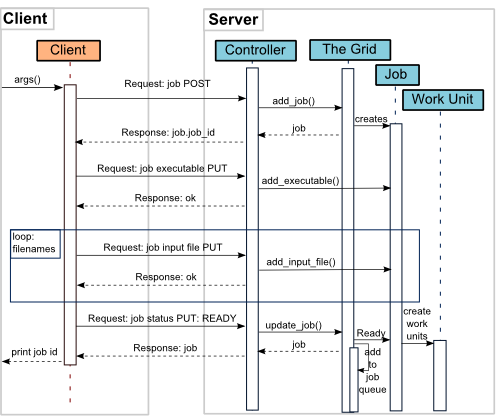
\includegraphics[keepaspectratio,width=\textwidth,height=0.75\textheight]{./figs/creation.png}
\caption{New Job Creation}
\end{figure}


\begin{figure}[htbp]
\centering
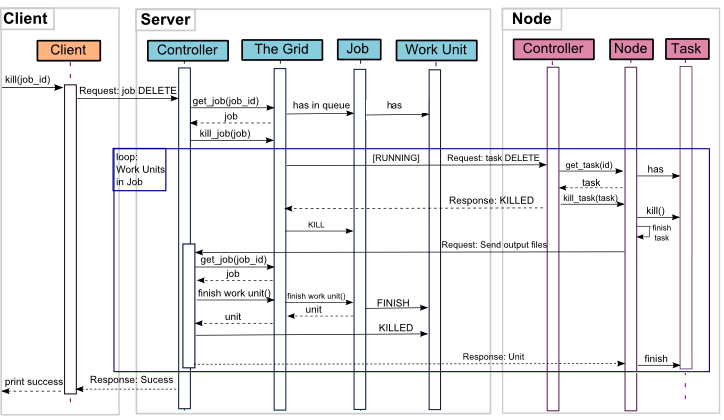
\includegraphics[keepaspectratio,width=\textwidth,height=0.75\textheight]{./figs/deletion.png}
\caption{Kill a Job}
\end{figure}


![Get the status of The Grid](.\slash figs\slash grid status.png)

![Get the status of a Job](.\slash figs\slash job get.png)

![Get the output of a finished Job](.\slash figs\slash output get.png)

\begin{figure}[htbp]
\centering
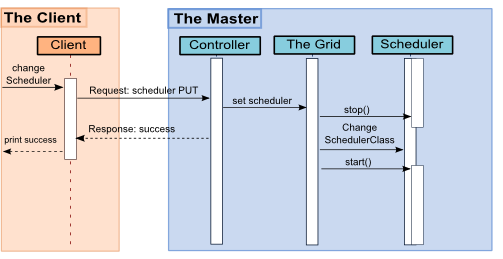
\includegraphics[keepaspectratio,width=\textwidth,height=0.75\textheight]{./figs/scheduler.png}
\caption{Change the scheduler dynamically}
\end{figure}


\begin{figure}[htbp]
\centering
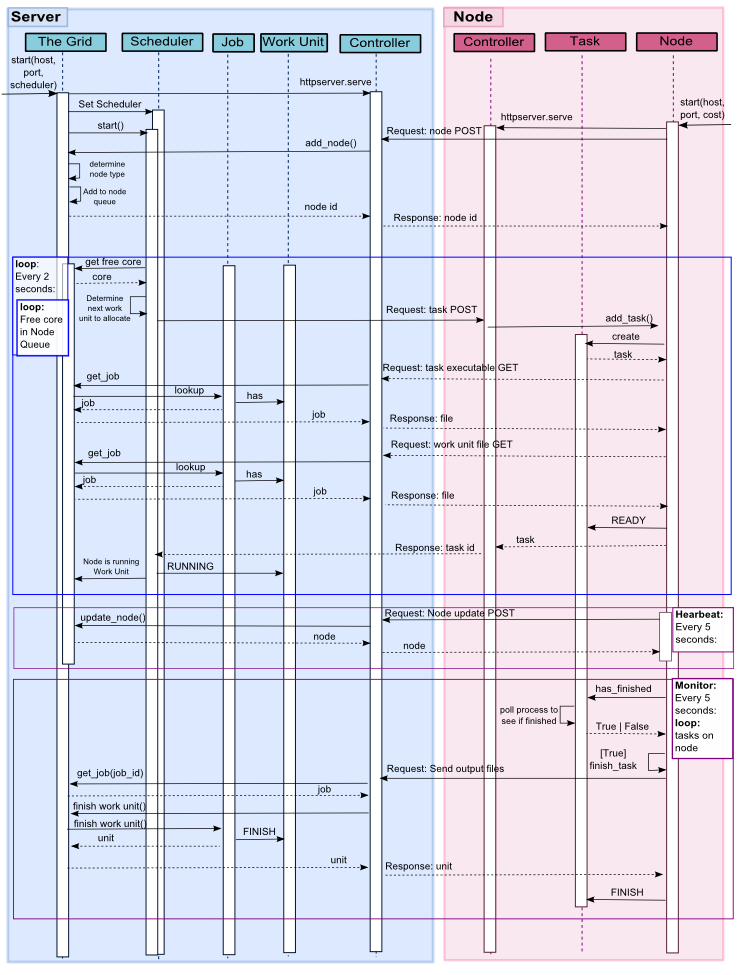
\includegraphics[keepaspectratio,width=\textwidth,height=0.75\textheight]{server-node.png}
\caption{Interaction between The Master and The Nodes in The Grid}
\end{figure}


\part{Implementation}
\label{implementation}

\chapter{Implementation}
\label{implementation}

The Grid is implemented using Python 2.6, with a package dependency on Paste. Paste is a multithreaded HTTP server which is used as the underlying communication protocol in The Grid. Communication between The Client and The Master, and The Master and The Nodes is done via an agreed JSON based API. 

Python 2.6 was chosen for both internal and external reasons. Internally, the development group all knew Python better than any other language which was suitable for the task. Secondly, development in Python is quite fast, though Python itself can be quite slow. As the main latency in The Grid is in the sending of input files and executables around, the computational speed loss due to language choice was deemed negligible. Externally, Python 2.6 was chosen due to its commonly installed nature which would make it easier to install The Node software on potential nodes. 

The dependency on an external library Paste was determined nessecary, though external libraries were avoided where possible. This was done to both avoid licensing issues, as well as making the software easier to install as it needed to be portable and installed on many different environments due to the heterogenous nature of The Grid. Neither of the WSGI servers available in the standard library of Python were suitable as neither is multi-threaded, which is unworkable due to having to send possibly large files around that would otherwise block the server from accepting new requests.

The choice of HTTP to communicate over was done so because of the familiarity of the development team with HTTP based communication protocols and the development of RESTful APIs with which to communicate via JSON over HTTP. It also allowed for the easy development of a web based GUI which both had the benefit of playing to the development teams strengths as well as allowing for a interface to The Grid that is accessible anywhere in the world via the internet. HTTP also has built in authentication which was utilised in order to provided a level of security for who can access and use The Grid. HTTP is also extendible to use HTTPS which would allow for the easy securing of communication within The Grid as a possible future extension of the software.

JSON specifically was chosen as it is light-weight and easier to parse than XML, while also being easily used from within JavaScript which allowed the web service on The Master to utilise the same RESTful API as the Client and Nodes do. 

The code was developed following the MVC style architecture, though as the majority of the views are actually JSON, the majority of the code is organised into Models and Controllers. Each of the web servers on The Master and The Nodes listen to a provided list of Routes which map URIs and request type (GET, POST, PUT, DELETE) to a controller which calls any specific functions from the model and returns the relevant output JSON.

\section{The Master}
\label{themaster}

The Master instansiates a HTTP Server on a given hostname and port, which it listens on for both communications from instances of The Client as well as web requests to the Graphical User Interface provided. The Master also uses this HTTP Server to accept messages from each of The Nodes in The Grid. 

\subsection{The Scheduler}
\label{thescheduler}

The Master contains a Scheduler, which runs inside its own thread. It periodically polls the internal node list to see if any nodes have become available. If a node is available, it will check to see if there are any Work Units available that can be run on that node. If there is a job available, then The Scheduler will allocate the Work Unit to that node. It will then continue looking at available nodes and attempting to find available Work Units for them. 

The Scheduler itself is itself contained within The Master and can be dynamically changed. In the case that a Scheduler is swapped however, the internal state unique to one Scheduler type will be lost and all jobs currently in the queue will be allocated using the new scheduling algorithm. The Scheduling algorithms available are: FCFS (First come, first served), Round Robin, Deadline First, Deadline\slash Cost First, and Mutli-level Priority Queues. 

\subsubsection{FCFS}
\label{fcfs}

FCFS completes each job sequentially as they arrived. Jobs are ordered by the time they were created, and all of the Work Units in a job will be completed before Work Units from another job are executed. If a job is created but is not ready (not all files have arrived on The Master) then a job that has been created later but is ready will be executed. When the earlier job becomes ready, all Work Units from the earlier job will be executed before resuming the job that was ready first but created later. This is done as to not unfairly punish jobs with large input files by making them wait until they are ready to be considered in the queue.

\subsubsection{Round Robin}
\label{roundrobin}

Round Robin is similar to FCFS however rather than executing all of the Work Units from a job before moving to the next one, it will instead execute one work unit from each job in the queue before moving on to the second work unit from each job in the queue. 

COMMENT ABOUT HOW JOBS ARE NOT STARVED OUT

\subsubsection{Deadline First}
\label{deadlinefirst}

Deadline First takes into account the deadline of the job and prioritises jobs by earliest deadline first. That is, if a job needs to be finished by tomorrow and there is another job that can be finished in a week, then the job that needs to be finsihed by tomorrow will take preference. As Jobs are allocated by schedulers as Work Units, a job may execute some work units before a Job is created that has an earlier deadline. In this event any remaining Work Units from the already running job will be placed behind the Work Units of the new scheduler. As a jobs deadline is a fixed amount of time in the past, indefinate starvation of a job cannot occur as eventually the deadline of the job will make it the highest priority to be completed. 

\subsubsection{Deadline\slash Cost First}
\label{deadlinecostfirst}

Deadline\slash Cost First takes into account not only the deadline of each Work Unit as in Deadline First but also takes into account the budget of the Job. It first ensures that a job only runs on nodes that are within the Jobs budget. It secondly preferentially places jobs with higher budgets about jobs with lower budgets. 

\subsubsection{Multi-level Priority Queues}
\label{multi-levelpriorityqueues}

This Multi-Level Priority Queue implementation splits The Nodes on The Grid into seperate queues. There can be any number of different queues, with a different proportion of The Grid allocated to them. The default queues are Default, Batch and Fast. Half of The Nodes on The Grid are allocated to Default, which is for any generic job between 1 hour and a few days. Batch is allocated 30\% of the nodes and is for jobs that will take a week or more. Fast is allocated 20\% of the nodes and is for jobs that are less than an hour. These priorities reserve nodes for specific job types without indefinately starving any one type of job if there is an excess of another.

This scheduler also stops large jobs from taking up most of the queue during offpeak periods, and then causing a large back log of other jobs. This is an unfortunate side effect of not being able to pause and resume a Work Unit once it has begun. While Deadline First and such can interupt a low priority job in terms of stopping further execution of additional work units, if a job is already running a number of work units which each may take a long time, there is no way to interrupt these running processes.

\section{The Node}
\label{thenode}

Each Node, like The Master, also instansiates a HTTP Server on a given hostname and port. It listens on this for communications from The Master. The Master sends job information to The Node, which in turn uses this information to request from The Master any files that The Node requires in order to complete the job it has been assigned.

\subsection{The Heartbeat}
\label{theheartbeat}

The Heartbeat is a thread spawned from The Node which controls the sending of the Node's heartbeat to The Master. This heartbeat lets The Master know that The Node is still there, if this heartbeat is not received by The Master, it will be assumed to be offline. This heartbeat also detects for a loss of connection to The Master. If connection to The Master is lost, The Node will attempt to reregister itself to The Master. 

\subsection{The Monitor}
\label{themonitor}

The Monitor is a thread spawned from The Node which monitors the health of The Node. It reports information such as the CPU usage to The Server so that overall statistics of The Grid can be monitored at a Grid-wide level.

\section{The Client}
\label{theclient}

A job has 3 various states throughout The Grid. On The Master it exists both as a Job, and as a number of Work Units which exist as part of a Job. A work unit is a pairing of the executable for a job and one input file. In the case of a job with 5 input files, it will have 5 work units, each corresponding to one input file. The level of granularity handled by The Scheduler is a single Work Unit. 

\chapter{The Grid: API}
\label{thegrid:api}

Both the Web based User Interface and the Client application (Client.py) communicate with the master node of The Grid through a REST API. REST stands for Representational State Transfer and is becoming the de-facto standard for web based API's, such as those used by Twitter and Facebook. The key benefits to using this technology are that many tools exist for consuming these services; it works over HTTP enabling consumption of services on mobile devices and provides a consistent model to develop with.

Rather than using XML, we have chosen to use the JSON format. The primary driver for selecting JSON is its simplicity. XML can easily become cumbersome for development due to the challenges of maintaining XML schemas in a rapidly evolving development process. JSON is also extremely well supported within Python and Javascript which greatly simplified development.

The REST API is secured using based HTTP Authentication, preventing unauthorized access to The Grid.

\section{API End Points}
\label{apiendpoints}

\subsection{Submit Job}
\label{submitjob}

The meta-data of a job must be submitted before files can be submitted and before the job can be started.

\begin{adjustwidth}{2.5em}{2.5em}
\begin{verbatim}

URL:    /job
Method: POST
Parameters: 
    name            label for identifying the job
    wall_time       time allowance for the job (HH:MM:SS)
    deadline        date and time that the job must be completed by
    budget          amount of money this job may cost
    job_type        type of job (BATCH, FAST, DEFAULT)
Returns:    
    job_id

\end{verbatim}
\end{adjustwidth}

\subsection{Submit Executable File}
\label{submitexecutablefile}

Only a single executable file may be uploaded to the server for a particular job. If multiple files are uploaded, then latter uploads will replace the initial file.

\begin{adjustwidth}{2.5em}{2.5em}
\begin{verbatim}

URL:    /json/job/submit-executable/<job_id>/?qqfile=<file_name>
Method: POST
Parameters: 
    job_id          the id of the job to submit the file to
    file_name       name of the executable file
    file_content    content of the file in the post body
Returns:    
    job_id, file_name

\end{verbatim}
\end{adjustwidth}

\subsection{Submit Input File}
\label{submitinputfile}

Many files may be associated with a single job, with the executable being executed with a single input file in each invocation which may occur on different servers.

\begin{adjustwidth}{2.5em}{2.5em}
\begin{verbatim}

URL:    /json/job/submit-file/<job_id>/?qqfile=<file_name>
Method: POST
Parameters: 
job_id          the id of the job to submit the file to
file_name       name of the executable file
file_content    content of the file in the post body
Returns:        job_id, file_name

\end{verbatim}
\end{adjustwidth}

\subsection{Start Job}
\label{startjob}

After all the required files have been uploaded, the job may be started using the above mentioned url.

\begin{adjustwidth}{2.5em}{2.5em}
\begin{verbatim}

URL:    /job/<job_id>/status
Method: POST
Parameters: 
job_id      the id of the job to start
status      must always be “READY”
Returns:

\end{verbatim}
\end{adjustwidth}

\subsection{Kill Job}
\label{killjob}

A job may be killed when it is Queued, Ready, Pending or Running, in which case all work items that have been queued or are running will be halted. The output for jobs that have already been run will still be available.

\begin{adjustwidth}{2.5em}{2.5em}
\begin{verbatim}

URL:    /job/<job_id>
Method: DELETE
Parameters: 
job_id      the id of the job to kill
Returns:

\end{verbatim}
\end{adjustwidth}

\subsection{List Available Nodes}
\label{listavailablenodes}

A list of all currently connected nodes is provided at this url along with the work items that each node is currently working on.
 URL: \slash json\slash nodes
 Method: GET
 Parameters:
 Returns: JSON encoded string listing available nodes.

\subsection{List Jobs}
\label{listjobs}

A list of all jobs that are in the pending, ready, queued, running, finished or killed state along with each jobs work items and the output files associated with those work items.

\begin{adjustwidth}{2.5em}{2.5em}
\begin{verbatim}

URL:    /json/jobs
Method: GET
Parameters:
Returns:    JSON encoded string listing jobs that have been submitted.

\end{verbatim}
\end{adjustwidth}

\part{Evaluation}
\label{evaluation}

\chapter{Evaluation}
\label{evaluation}

\part{Future Improvements}
\label{futureimprovements}

\chapter{Future Improvements}
\label{futureimprovements}

 \clearpage \chapter{Contributions}
\label{contributions}

Each team member of the group has contributed approximately 25\% of the work to this project. Specific leading contributions of each team member are outlined below, however all team members contributed to all aspects of the developement and design of The Grid. 

\textbf{Adam Whiteside \& Scott Richie} - Backend Communication and Framework

\textbf{Terence Siganakis} - Graphical User Interface

\textbf{Andrew Vadnal} - Scheduling Algorithms

\input{mmd-memoir-footer}

\end{document}
